
\documentclass[english]{article}
\usepackage[utf8]{inputenc}
\usepackage[margin=1in]{geometry}
\usepackage{graphicx,wrapfig,lipsum}
\usepackage{caption}
\usepackage{refstyle}
\usepackage{titlepic}
\usepackage{graphicx}
\usepackage{grffile}
\usepackage{babel}
\usepackage{parskip}
\usepackage{hyperref}
\textwidth = 426pt
\oddsidemargin = 17pt


\title{Cos301 : Test Policy\\
	for the SmartCard Application\\
}
\date{\today}
\graphicspath{{Pictures/}}

\begin{document}
	\maketitle
	\begin{figure}[!t]
		
\includegraphics{up_logo.png}
	\end{figure}
	\begin{minipage}{0.4\textwidth}
		\begin{flushleft} \large
			\textbf{NAMES:}\\[0.4cm]
			Mufamadi {Khodani} \\
			Setoaba {Phuti} \\
			Dandashe {Kagiso Xolo} \\
			
		\end{flushleft}
	\end{minipage}
	\begin{minipage}{0.4\textwidth}
		\begin{flushright} \large
			\textbf{STUDENT NUMBER:} \\[0.4cm]
			u14197520 \\
			u13032616 \\
			u14245681 \\
		\end{flushright}
	\end{minipage}
	
	
	\pagenumbering{gobble}
	\newpage
	
	\tableofcontents
	
	
	\pagenumbering{arabic}
	
	\newpage

	


	\pagenumbering{arabic}
	

	\section{Mission of Testing}
	To effectively deliver efficient and effective software that meets the customers requirements. To further ensure that quality software is produced.  


	\section{Test Description}
	
	We include three categories of tests:
	
		\begin{itemize} 
			\item Small tests which are unit tests that you can run in isolation from production systems. They typically mock every major component and should run 				quickly on your machine.
			\item Medium tests which are integration tests that sit in between small tests and large tests. They integrate several components, and they run on 						emulators or real devices.
			\item Large tests which are integration and UI tests that run by completing a UI workflow. They ensure that key end-user tasks work as expected on 						emulators or real devices.
		\end{itemize}
		Our Testing process will be divided into two sections. Unit testing and Automated testing. 
		\begin{itemize} 
			\item Unit testing is done using Junit
			\item Automated testing is done using Espresso
		
		\end{itemize}
	We choose to use Espresso because it is free and easily intergratable or comes built in with android studio which is the platform we are using to develop our app ,and it also works hand-in-hand with jUnit so we can simply automate our junit unit tests to automated tests with a small configuration or change to the test code.
			

	
	\subsection {Unit testing}
			\subsubsection{Storage}
		\begin{itemize} 
			\item Check if the information is stored correctly.
			\item Check if the information can be retrieved from the database.
		\end{itemize}
			\subsubsection{Application activities and functions}
			\begin{itemize}
				\item Ensure that an appointment can be set and retrived
				\item Validate that emails are of the correct form 
				\item Ensure that a user can be created
			\end{itemize}
	
	\subsection {Test Cases}
	Below are our tests which are grouped by Large Automated tests which consist of the listed Unit tests within them
		\subsubsection{Incorrect Log In functionality}
		\begin{itemize} 
			\item test for when No input is entered to the email and and password field
			\item test for when only the email is provided 
			\item test for when the email and password  are both incorrect
			\item test for when correct email is provided and incorrect password
			\\
			\href{url}{https://github.com/XoloKDandashe/Alpha-Tech/blob/master/Code/NFCBusinessCardLocal2/app/src/androidTest/java/com/example/www/nfcbusinesscardlocal/LogInIncorrectDetails.java}

		\end{itemize}
		\subsubsection{Correct Log In And functionality}
		\begin{itemize} 
			\item tests if a Registered User can login to the app
			\item tests if a user can logout after a successful login
			\item tests if the App displays a message to warn the user that they are about to log out
			\\
			\href{url}{https://github.com/XoloKDandashe/Alpha-Tech/blob/master/Code/NFCBusinessCardLocal2/app/src/androidTest/java/com/example/www/nfcbusinesscardlocal/CorrectLogInandLogOutTest.java}
		\end{itemize}

		\subsubsection{Register And LogIn functionality}
		\begin{itemize} 
			\item Checks if a new user can register an account
			\item Checks if passwords match when confirming password when registering
			\item Checks if a new user can Log in with their details 
			\\
	\href{url}{https://github.com/XoloKDandashe/Alpha-Tech/blob/master/Code/NFCBusinessCardLocal2/app/src/androidTest/java/com/example/www/nfcbusinesscardlocal/RegisterNewUserAndLogInTest.java}

			
		\end{itemize}
		\subsubsection{Generate QR Code functionality}
			\begin{itemize} 
				\item Checks if the generate Qr Code button works
				\item Check if the QR code generates correct information
				\\
					\href{url}{https://github.com/XoloKDandashe/Alpha-Tech/blob/master/Code/NFCBusinessCardLocal2/app/src/androidTest/java/com/example/www/nfcbusinesscardlocal/GenerateQRCodeTest.java}

			\end{itemize}
	\subsubsection{Scan QR Code functionality}
			\begin{itemize} 
				\item Checks if the Scan QR code button works
				\item Checks if the Scan QR code button opens the camera intent
				\item Checks if the Qr code is scanned and the user information is displayed and saved
\\
					\href{url}{https://github.com/XoloKDandashe/Alpha-Tech/blob/master/Code/NFCBusinessCardLocal2/app/src/androidTest/java/com/example/www/nfcbusinesscardlocal/QrScannerTest.java}
			\end{itemize}
		\subsubsection{View Details functionality}
			\begin{itemize} 
				\item Checks if the view details button works
				\item Checks if the view details activity displays the current user information
\\
					\href{url}{https://github.com/XoloKDandashe/Alpha-Tech/blob/master/Code/NFCBusinessCardLocal2/app/src/androidTest/java/com/example/www/nfcbusinesscardlocal/ViewUserDetailsTest.java}
			\end{itemize}
		\subsubsection{Update user details functionality}
			\begin{itemize} 
				\item Checks if the update user details button works
				\item tests if the user can update thier information
\\
					\href{url}{https://github.com/XoloKDandashe/Alpha-Tech/blob/master/Code/NFCBusinessCardLocal2/app/src/androidTest/java/com/example/www/nfcbusinesscardlocal/UpdateUserDetailsTest.java}
			\end{itemize}
		\subsubsection{NFC functionality}
		\begin{itemize} 
			\item Tests if the App notifies the user if the NFC technology is not switched on.
			\item Tests if the App notifies users that do not have NFC
\\
					\href{url}{}
			
		\end{itemize}
		\subsubsection{View Cards Functionality}
		\begin{itemize}
			\item Tests whether a user can view thier saved cards
			\item Tests the functionality of the search tool that searches for saved card
			\item Tests if a user can delete a saved card
			\item Tests if a user can view the details of a saved card
\\
					\href{url}{https://github.com/XoloKDandashe/Alpha-Tech/blob/master/Code/NFCBusinessCardLocal2/app/src/androidTest/java/com/example/www/nfcbusinesscardlocal/ViewCardsTest.java}
		\end{itemize}
		\subsubsection{NFC Send functionality}
		\begin{itemize} 
			\item Tests the Nfc send function and if it sends correct information
\\
					\href{url}{}
		\end{itemize}

		\subsubsection{Import Card Functionality}
		\begin{itemize}
			\item Tests whether the import card button works
			\item Tests whether the capture card button opens the camera intent
\\
					\href{url}{}
		\end{itemize}
		\subsubsection{Create and View Appointment Functionality}
		\begin{itemize}
			\item Tests whether a user can Create an Appointment
			\item Tests whether a user can view saved Appointments
			\item Tests whether a user can delete an appointment
\\
					\href{url}{}
		\end{itemize}
		\subsubsection{Navigation Functionality}
		\begin{itemize}
			\item Tests if the navigate me button opens the google maps API
			\item Tests if the find me button returns the current locaton or an error message if it couldnt find the location
\\
					\href{url}{}
		\end{itemize}
		
			
	
		

	\section{Test Evaluation}
	
	We will use JUnit and  Espresso to ensure that implementations have been functions as it should.
	Espresso automates tests ,  JUnit is a testing framework for Android and Java applications.
	\section{Quality level to be achieved}
	We aim to have no outstanding faults prior to product release.
	
	\section{Approach to Test process improvement}
	
	Project review meetings are held in regards to improving the project.
	
	
	 
	\section{Git test cases  }
	link to the github test cases folder

					\href{url}{https://github.com/XoloKDandashe/Alpha-Tech/tree/master/Code/NFCBusinessCardLocal2/app/src/androidTest/java/com/example/www/nfcbusinesscardlocal}
	\section{History}
	snapshot of some test cases
\begin{figure}[h!]
				\centering
			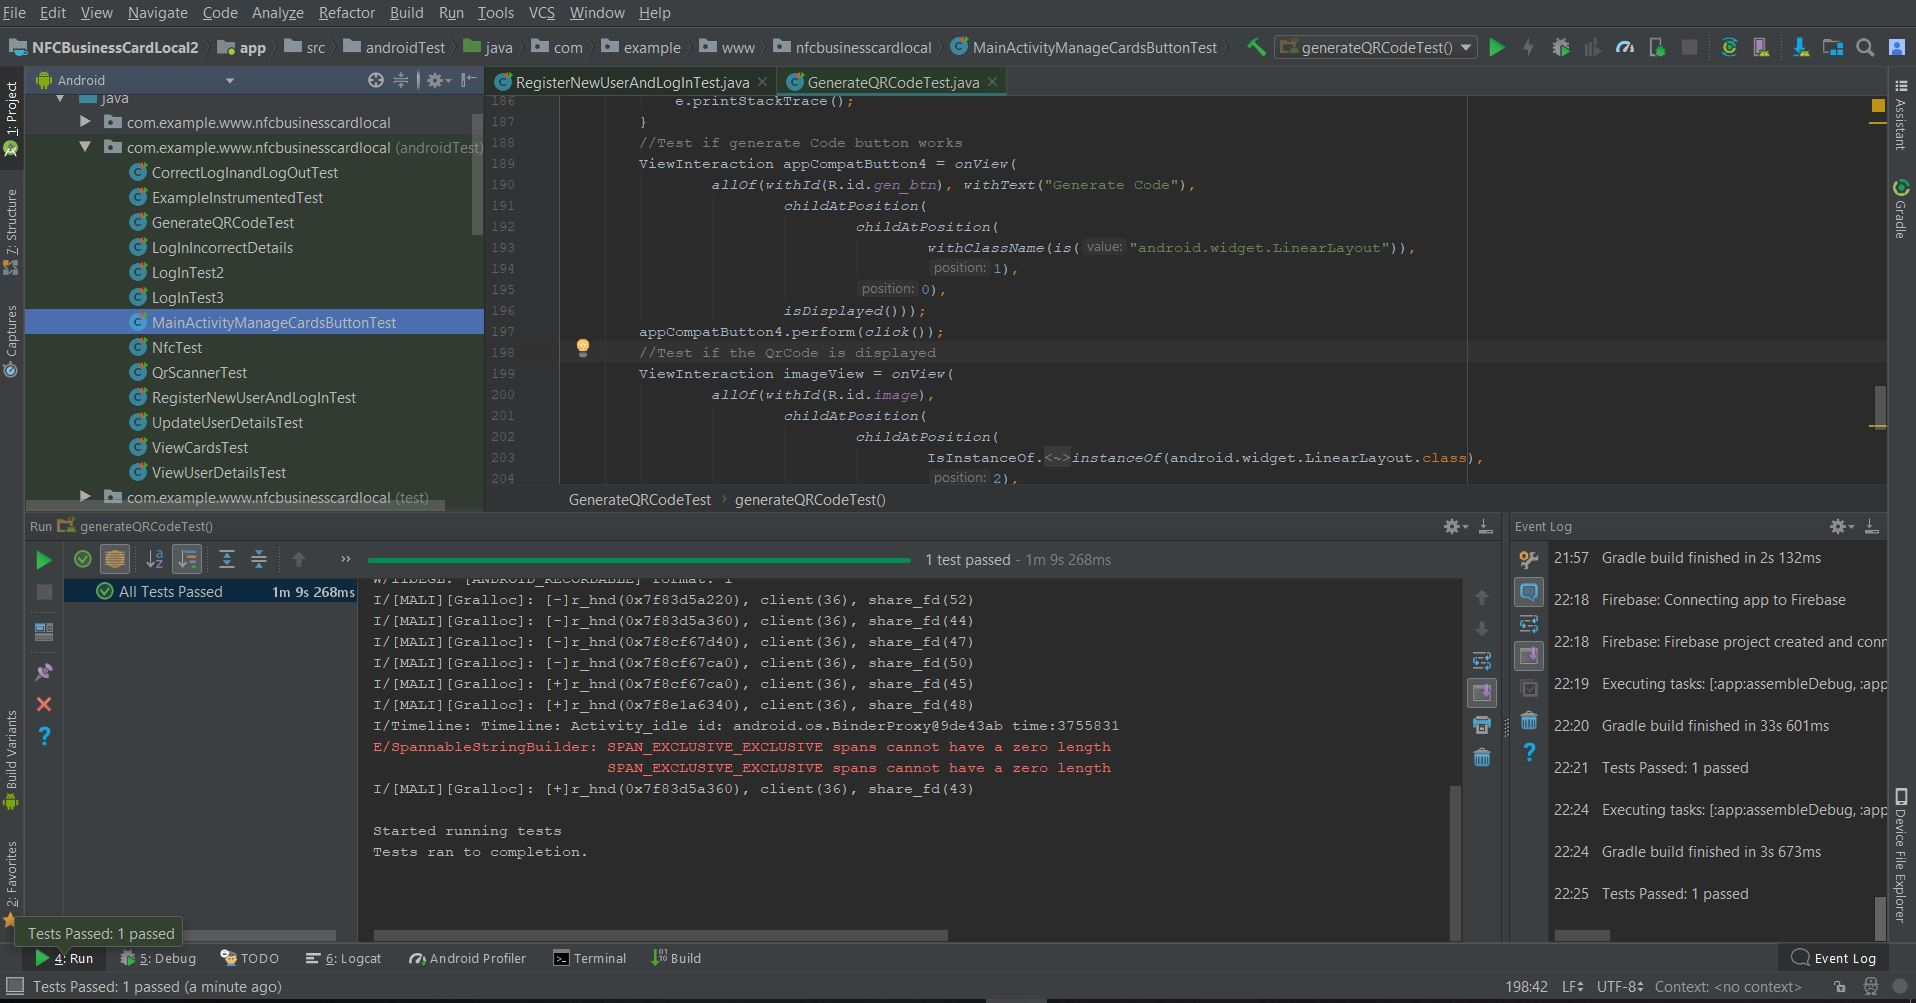
\includegraphics[scale=0.7]{Capture.jpg}
				\caption{GenerateQr test pass}
				\label{figure: 1}
			\end{figure}
			%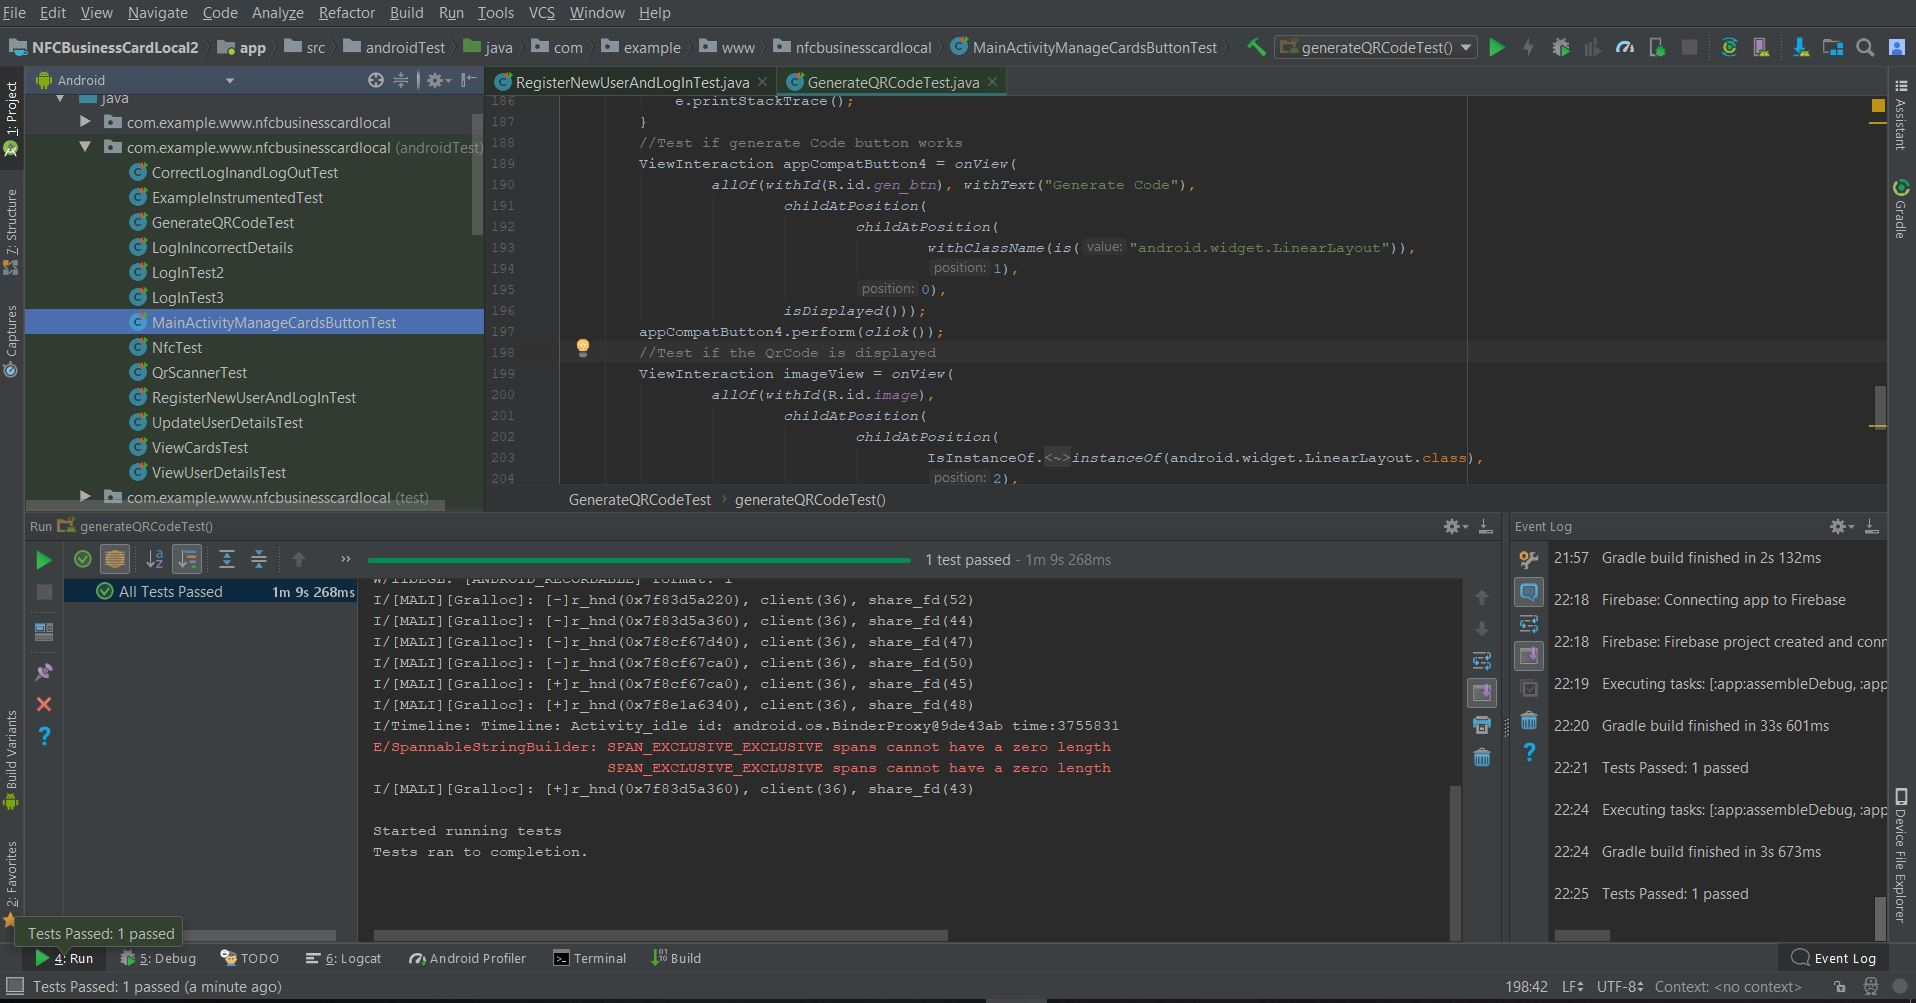
\includegraphics[scale=0.7]{Capture.jpg}
\begin{figure}
				\centering
			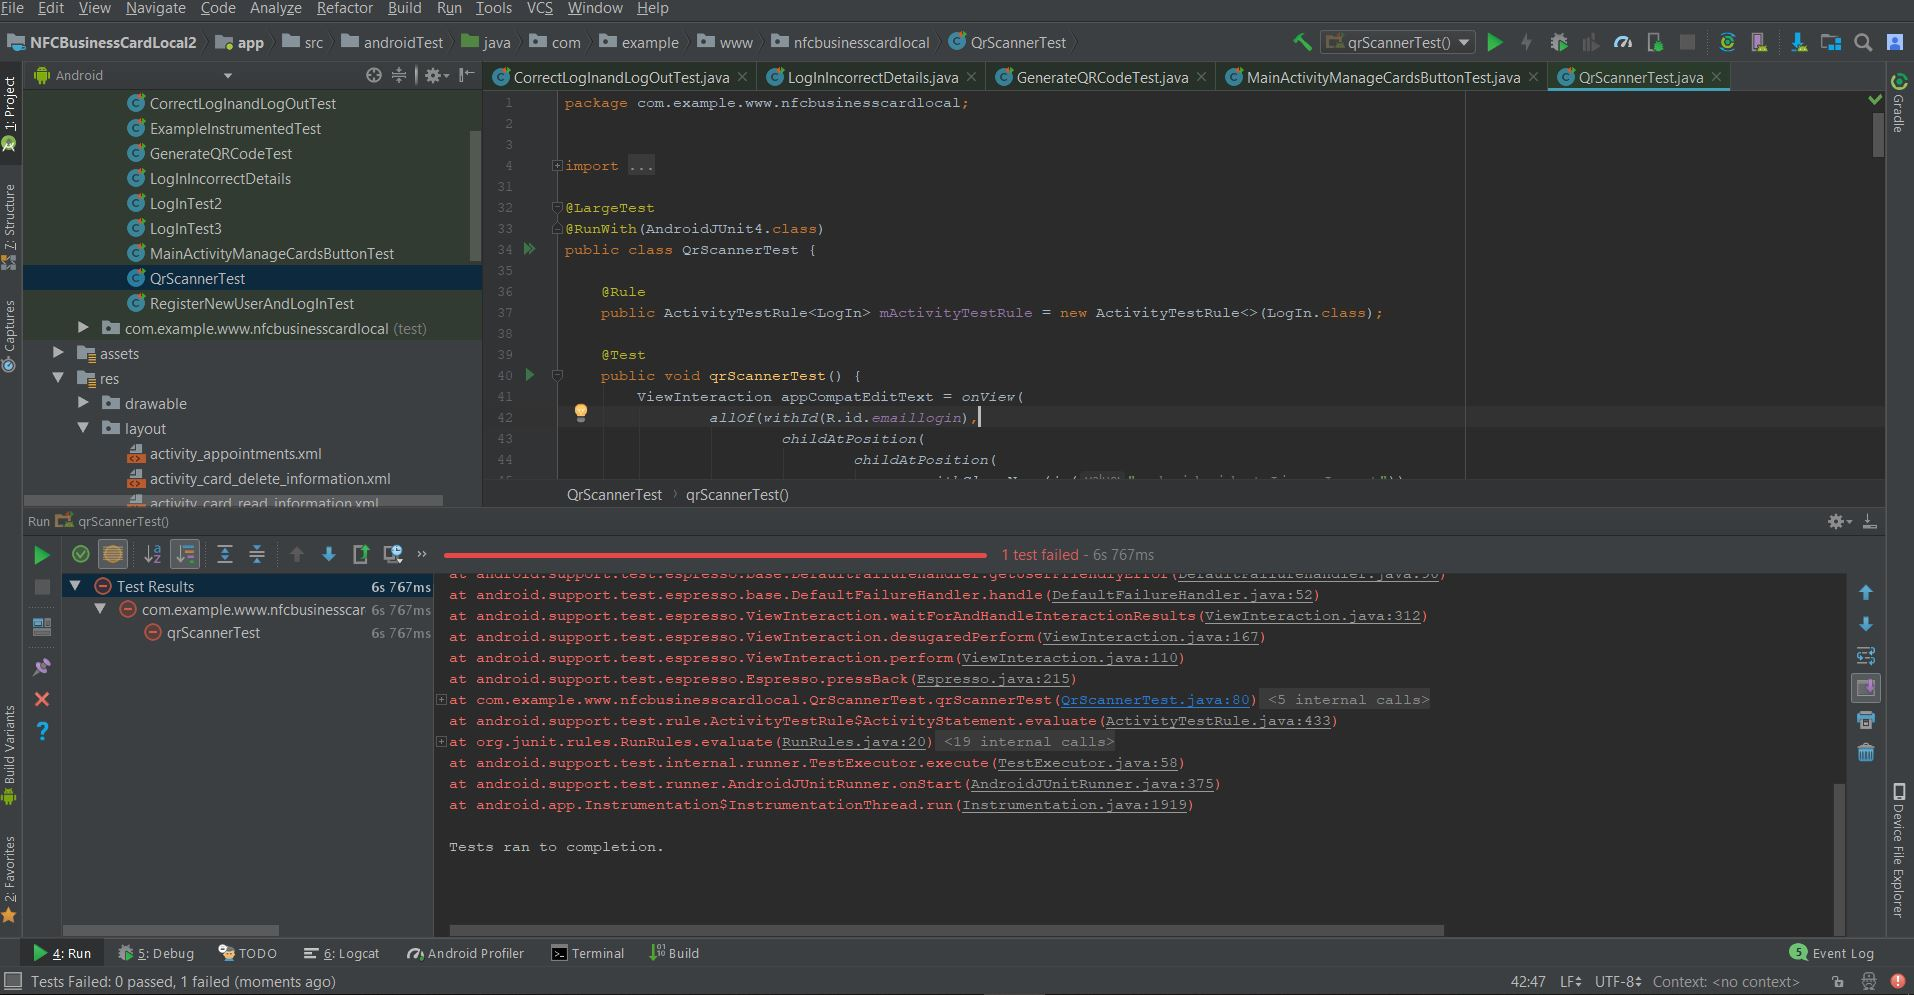
\includegraphics[scale=0.7]{QrscanFail.jpg}
				\caption{Qrscan test fail}
				\label{figure: 1}
			\end{figure}
			%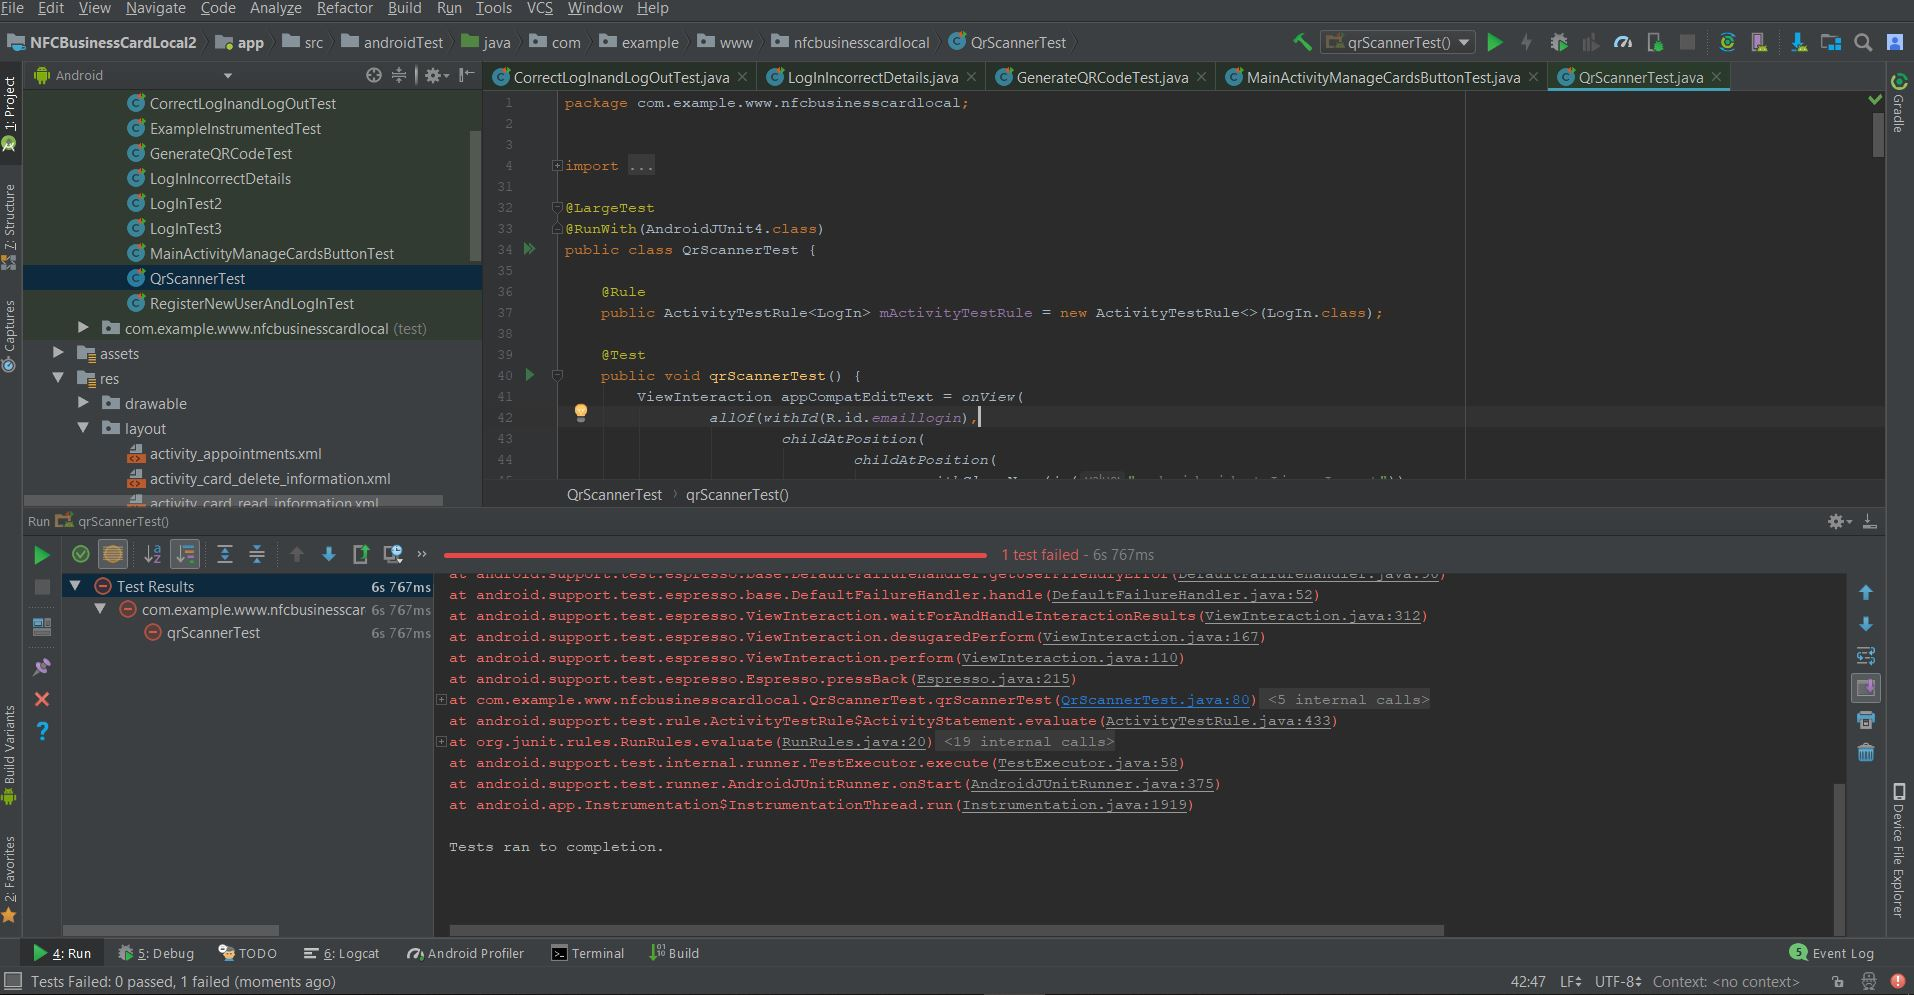
\includegraphics[scale=0.7]{QrscanFail.jpg}
\begin{figure}
				\centering
			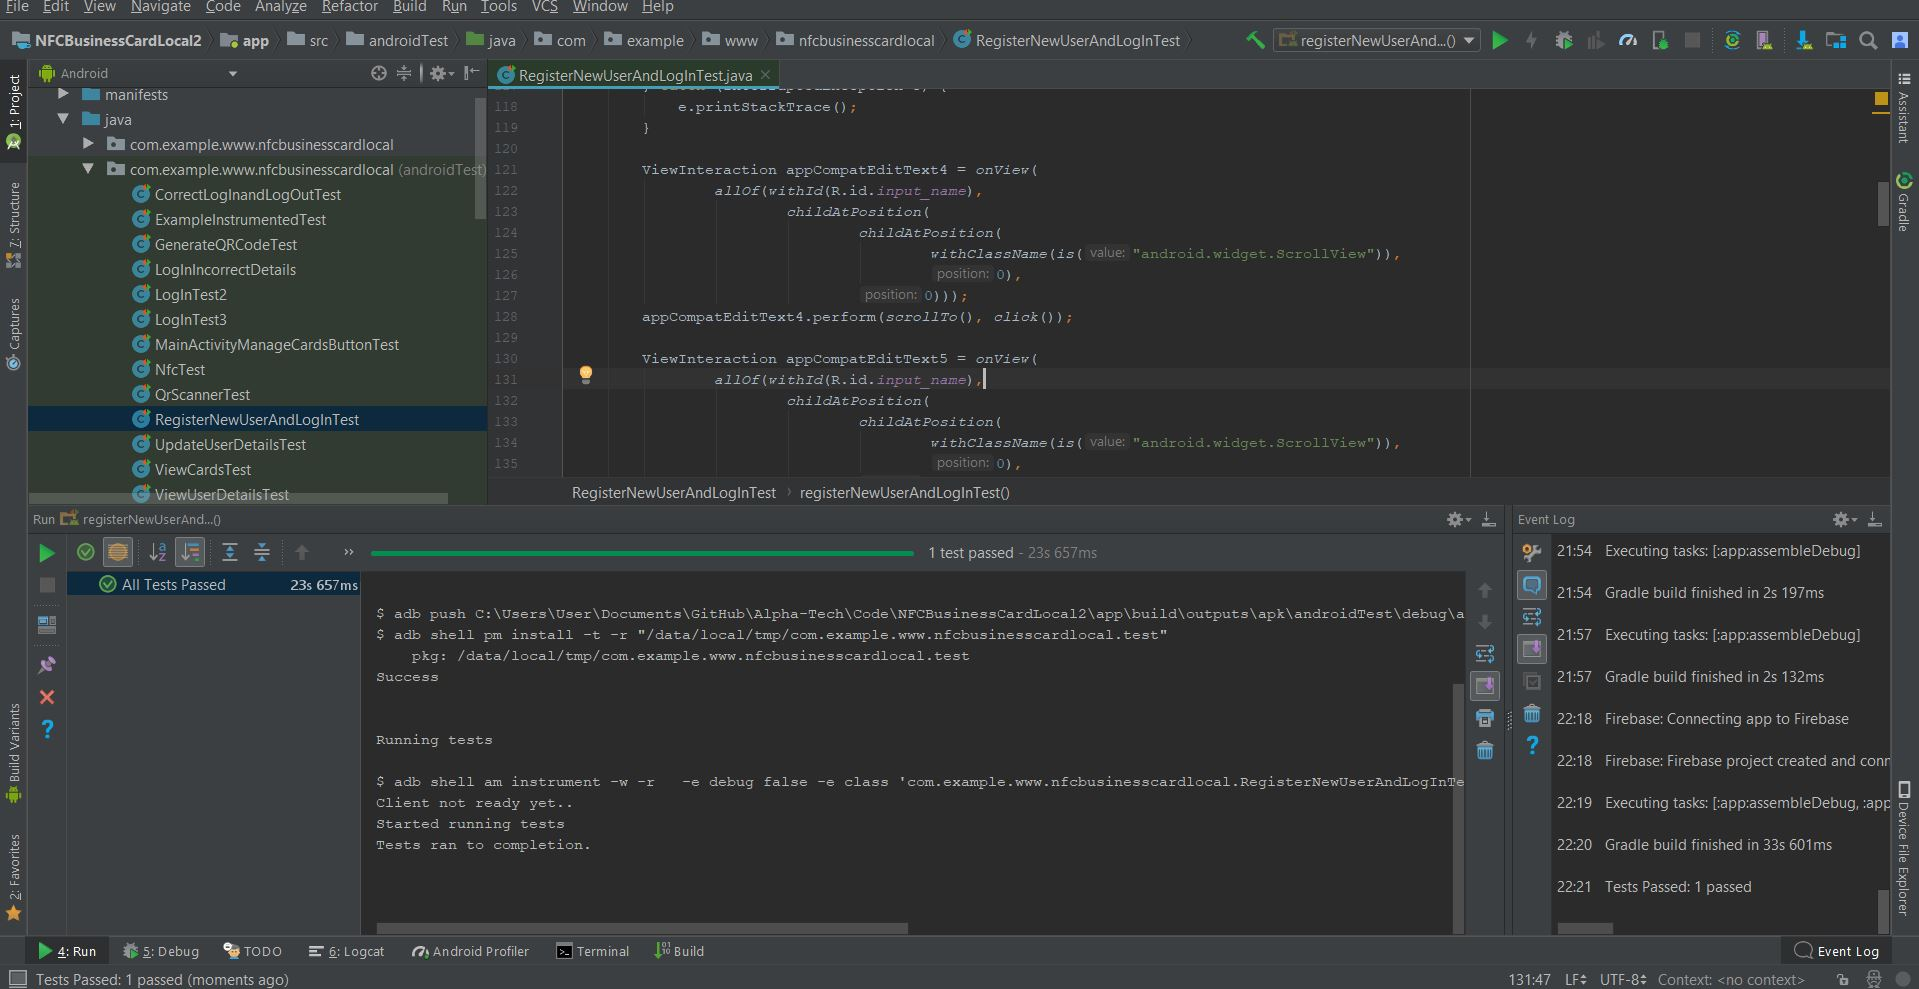
\includegraphics[scale=0.7]{RegisterTest.jpg}
				\caption{Register new user And login test pass}
				\label{figure: 1}
			\end{figure}
			%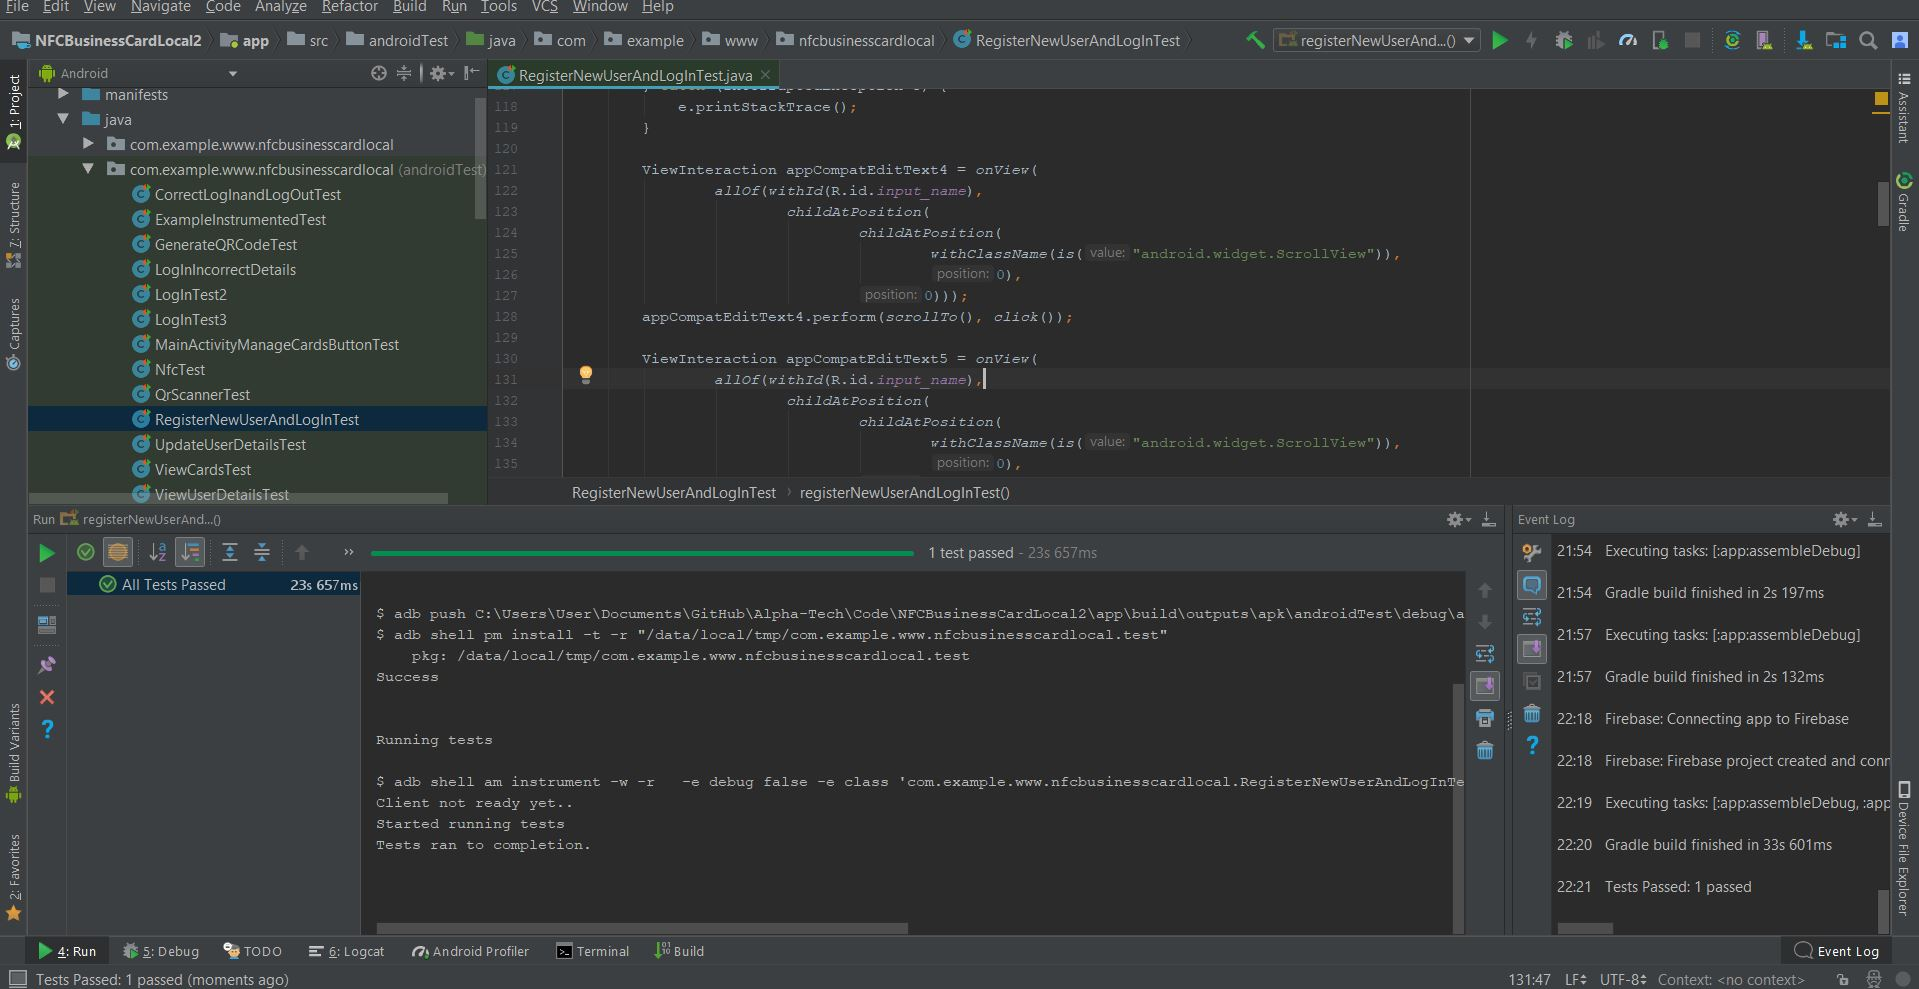
\includegraphics[scale=0.7]{RegisterTest.jpg}


	
	
		
\end{document}
